\documentclass[a4paper,11pt,openany]{book}

\usepackage{tt100}
\usepackage{pgf,tikz}
\usetikzlibrary{arrows}
\usetikzlibrary{decorations.pathreplacing}
\pagestyle{plain}

%Linkit sis�llysluetteloon
\usepackage{color}
\usepackage[hidelinks]{hyperref}
\hypersetup{colorlinks, urlcolor = blue, linkcolor = black, citecolor = black}%allcolors=black}

\hyphenation{o-sa-jouk-ko sis�-tulo-ava-ruu-den o-sa-jou-kot o-sa-jou-kok-si o-sa-jouk-ko-ja al-ku-as-ke-lees-sa}

%\includeonly{15_vektoriavaruus,16_aliavaruus,17_vapaus,18_kanta,19_lineaarikuvaus,20_ydinJaKuva,21_isomorfismi,22_kantaJaLineaarikuvaukset,23_lineaarikuvauksienOminaisarvot,24_sisatulo}

\begin{document}

\frontmatter
\begin{titlepage}

\begin{center}

\mbox{ }

\vspace{5.0cm}

{\bf \Huge Vektorit }


%\vspace{0.4cm}

%{\bf \Huge yliopistomatematiikkaan}

\vspace{2.0cm}

{\large Juulia Lahdenper� ja Lotta Oinonen}

\vspace{2.0cm}

\today \\

\end{center}

%\vfill
%\begin{flushright}
%Helsingin yliopisto\\
%Matematiikan ja tilastotieteen laitos
%\end{flushright}

\end{titlepage}

\thispagestyle{empty}
\cleardoublepage

\setcounter{page}{0}
%\pagestyle{empty}

%\thispagestyle{empty}
\tableofcontents

\setcounter{page}{0}
\mainmatter

\section{Vektori}


\subsection{Vektorit ja $xy$-koordinaatisto}

Kuvassa \ref{kuva:koordinaatiston nelj�nnekset} on koordinaatisto, johon on piirretty $x$- ja $y$-akselit. Koordinaattiakselit jakavat tason nelj��n osaan. Osat nimet��n yleens� j�rjestysnumeroilla I, II, III ja IV kuvan \ref{kuva:koordinaatiston nelj�nnekset} mukaisesti. Koordinaattiakselien leikkauskohtaa kutsutaan \textbf{origoksi}. Origoa merkit��n yleens� kirjaimella $O$. 

	\begin{center}
	\begin{figurehere}
	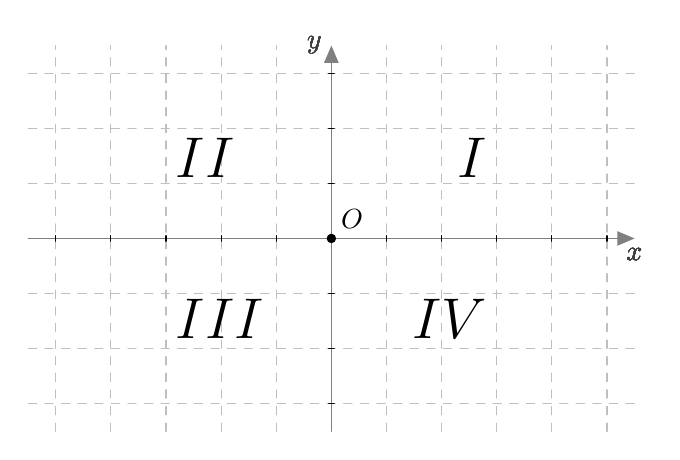
\begin{tikzpicture}[line cap=round,line join=round,>=triangle 45,x=0.7cm,y=0.7cm]

		%x-akseli:
		\draw[->,color=gray] (-5.5,0) -- (5.5,0);
		%tiksut ja viivat
		\foreach \x in {-5,-4,-3,-2,-1,1,2,3,4,5}
		{\draw[dashed, color= lightgray] (\x,-3.5)--(\x,3.5);
		\draw[shift={(\x,0)},color=black] (0pt,1pt) -- (0pt,-1pt);
		\node [below] at (5.5,0) {\textcolor{darkgray}{$x$}};
		}

		%y-akseli
		\draw[->,color=gray] (0,-3.5) -- (0,3.5);

		%tiksut ja viivat
		\foreach \y in {-3,-2,-1,1,2,3}
		{
		\draw[dashed, color=lightgray] (-5.5,\y)--(5.5,\y);
		\draw[shift={(0,\y)},color=black] (1pt,0pt) -- (-1pt,0pt);
		\node [left] at (0,3.5) {\textcolor{darkgray}{$y$}};
		}

		% Varsinainen kuva

		\node[below left] at (3,2) {\huge{$I$}};

		\node[below right] at (-3,2) {\huge{$II$}};

		\node[above right] at (-3,-2) {\huge{$III$}};

		\node[above left] at (3, -2) {\huge{$IV$}};
		
		\draw[fill, color = black] (0,0) circle [radius = 1.5pt];
		\node[above right] at (0,0) {$O$};

	\end{tikzpicture}
	\caption{Koordinaatiston nelj�nnekset.}
	\label{kuva:koordinaatiston nelj�nnekset}
	\end{figurehere}
	\end{center}	
		
\begin{teht} Tutki alla olevaa kuvaa \ref{kuva:kolme pistetta koordinaatistossa}. 
	
	\begin{center}
	\begin{figurehere}
	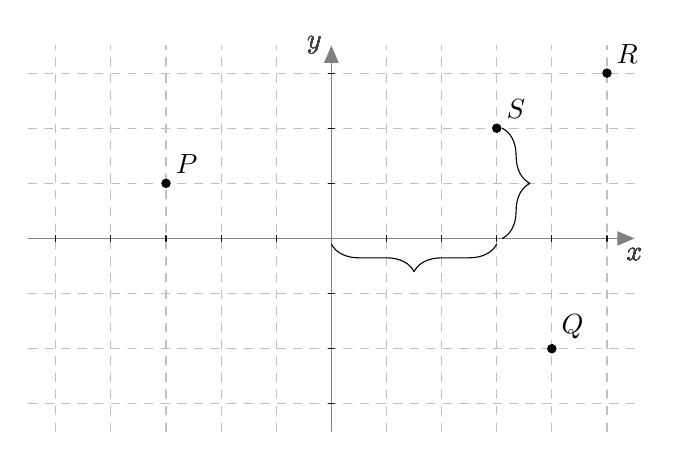
\begin{tikzpicture}[line cap=round,line join=round,>=triangle 45,x=0.7cm,y=0.7cm]

		%x-akseli:
		\draw[->,color=gray] (-5.5,0) -- (5.5,0);
		%tiksut ja viivat
		\foreach \x in {-5,-4,-3,-2,-1,1,2,3,4,5}
		{\draw[dashed, color= lightgray] (\x,-3.5)--(\x,3.5);
		\draw[shift={(\x,0)},color=black] (0pt,1pt) -- (0pt,-1pt);
		\node [below] at (5.5,0) {\textcolor{darkgray}{$x$}};
		}

		%y-akseli
		\draw[->,color=gray] (0,-3.5) -- (0,3.5);

		%tiksut ja viivat
		\foreach \y in {-3,-2,-1,1,2,3}
		{
		\draw[dashed, color=lightgray] (-5.5,\y)--(5.5,\y);
		\draw[shift={(0,\y)},color=black] (1pt,0pt) -- (-1pt,0pt);
		\node [left] at (0,3.5) {\textcolor{darkgray}{$y$}};
		}

		% Varsinainen kuva

		\draw[fill, color = black] (3,2) circle [radius = 1.5pt];
		\node[above right] at (3,2) {$S$};

		\draw[fill, color = black] (-3,1) circle [radius = 1.5pt];
		\node[above right] at (-3,1) {$P$};

		\draw[fill, color = black] (4,-2) circle [radius = 1.5pt];
		\node[above right] at (4, -2) {$Q$};
		
		\draw[fill, color = black] (5,3) circle [radius = 1.5pt];
		\node[above right] at (5, 3) {$R$};

		% Kaarisulku alasp.
		\draw [decorate,decoration={brace,amplitude=10pt,raise=2pt},yshift=0pt,rotate around={90:(3,0)},=90]
		(3,0) -- (3,3) node [black,midway,yshift=-0.7cm]{};

		% Kaarisulku oikeanp.
		\draw [decorate,decoration={brace,amplitude=10pt,mirror,raise=2pt},xshift=0pt]
		(3,0) -- (3,2) node [black,midway,xshift=0.7cm] {};

	\end{tikzpicture}
	\caption{Pisteit� koordinaatistossa.}
	\label{kuva:kolme pistetta koordinaatistossa}
	\end{figurehere}
	\end{center}
	
\begin{aakkosta*}
\item Kuinka monta yhden ruudun mittaista askelta pit�� siirty� $x$-akselin suunnassa, jotta p��st��n origosta pisteeseen $S$? 
\item Kuinka monta yhden ruudun mittaista askelta pit�� siirty� $y$-akselin suunnassa, jotta p��st��n origosta pisteeseen $S$? 
\item Kuinka monta yhden ruudun mittaista askelta pit�� siirty� $x$-akselin suunnassa, jotta p��st��n origosta pisteeseen $Q$? 
\item Kuinka monta yhden ruudun mittaista askelta pit�� siirty� $y$-akselin suunnassa, jotta p��st��n origosta pisteeseen $Q$? 
\item Miten voisit merkit� sit�, ett� pisteen $Q$ tapauksessa siirryt��n $y$-akselin suunnassa alas- eik� yl�sp�in, kuten pisteen $S$ tapauksessa?
\end{aakkosta*}
\end{teht}

Tason piste ilmoitetaan lukuparina $(x,y)$, miss� ensimm�inen luku $x$ ilmoittaa $x$-akselin suuntaisten ja toinen luku $y$ ilmoittaa $y$-akselin suuntaisten askelten lukum��r�n. N�it� lukuja kutsutaan \textbf{pisteen koordinaateiksi}. Kuvan \ref{kuva:kolme pistetta koordinaatistossa} pisteeseen $R$ p��st��n siirtym�ll� origosta viisi askelta $x$-akselin suuntaan ja kolme askelta $y$-akselin suuntaan. N�in ollen pistett� $R$ merkit��n $R=(5,3)$. Pistett� $P$ merkit��n puolestaan $P=(-3,1)$.

\begin{teht} Valitse jokaiselta koordinaatiston nelj�nneksell� jokin piste ja ilmoita sen koordinaatit. Miten eri nelj�nnekset vaikuttavat $x$- ja $y$-koordinaattien koordinaattien etumerkkeihin? 
\end{teht}	
	
\begin{teht} ...
\begin{aakkosta*}
\item Piirr� koordinaatisto ja merkitse siihen pisteet $(1,2)$, $(1,-4)$ ja $(1,3)$.
\item Merkitse piirt�m��si koordinaatistoon kolme uutta pistett�, jotka ovat muotoa $(1,y)$ jollakin kokonaisluvulla $y$.
\item Merkitse piirt�m��si koordinaatistoon kaikki sellaiset tason pisteet, jotka ovat muotoa $(1,y)$ jollakin kokonaisluvulla $y$. 
\end{aakkosta*}
\end{teht}

\begin{teht} ...
\begin{aakkosta*}
\item Piirr� koordinaatisto ja merkitse siihen pisteet $(2,2)$, $(3,3)$ ja $(-2,-2)$.
\item Merkitse piirt�m��si koordinaatistoon kolme uutta pistett�, jotka ovat muotoa $(x,x)$ jollakin reaaliluvulla $x$.
\item Merkitse piirt�m��si koordinaatistoon kaikki sellaiset tason pisteet, jotka ovat muotoa $(x,x)$ jollakin reaaliluvulla $x$. 
\end{aakkosta*}
\end{teht}
	
\begin{teht} Piirr� koordinaatisto ja merkitse siihen kaikki sellaiset tason pisteet, jotka ovat muotoa $(x,2/3)$ jollakin reaaliluvulla $x$. 
\end{teht}

Tarkastellaan seuraavaksi kuvaa \ref{kuva:vektorin muodostaminen}. Vasemmanpuoleisessa kuvassa on n�kyviss� koordinaattiakselien suuntaiset yhden yksik�n mittaiset vektorit $\vi$ ja $\vj$. Oikeanpuoleisessa kuvassa n�kyv�t vektorit $\vu, \vv$ ja $\vw$.

	\begin{center}
	\begin{figurehere}
	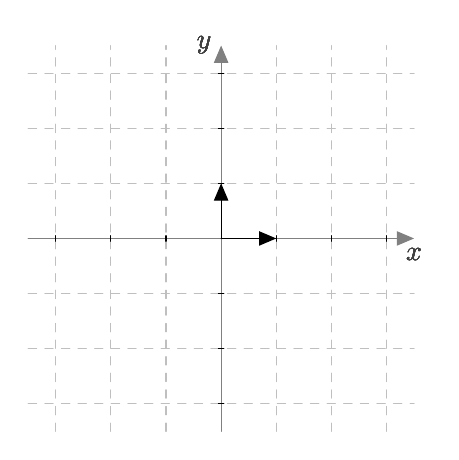
\begin{tikzpicture}[line cap=round,line join=round,>=triangle 45,x=0.7cm,y=0.7cm]

		%x-akseli:
		\draw[->,color=gray] (-3.5,0) -- (3.5,0);
		%tiksut ja viivat
		\foreach \x in {-3,-2,-1,1,2,3}
		{\draw[dashed, color= lightgray] (\x,-3.5)--(\x,3.5);
		\draw[shift={(\x,0)},color=black] (0pt,1pt) -- (0pt,-1pt);
		\node [below] at (3.5,0) {\textcolor{darkgray}{$x$}};
		}
		
		%y-akseli
		\draw[->,color=gray] (0,-3.5) -- (0,3.5);

		%tiksut ja viivat
		\foreach \y in {-3,-2,-1,1,2,3}
		{
		\draw[dashed, color=lightgray] (-3.5,\y)--(3.5,\y);
		\draw[shift={(0,\y)},color=black] (1pt,0pt) -- (-1pt,0pt);
		\node [left] at (0,3.5) {\textcolor{darkgray}{$y$}};
		}

		% Varsinainen kuva

		% Komponenttivektorit
		\draw[->] (0,0)--(1,0);
		\node[below] at (0.4, -0.2) {$\vi$};

		\draw[->] (0,0)--(0,1);
		\node[left] at (-0.2, 0.4) {$\vj$};

	\end{tikzpicture}
	\hspace*{0.7cm}
	\begin{tikzpicture}[line cap=round,line join=round,>=triangle 45,x=0.7cm,y=0.7cm]

		%x-akseli:
		\draw[->,color=gray] (-4.5,0) -- (5.5,0);
		%tiksut ja viivat
		\foreach \x in {-4,-3,-2,-1,1,2,3,4,5}
		{\draw[dashed, color= lightgray] (\x,-3.5)--(\x,3.5);
		\draw[shift={(\x,0)},color=black] (0pt,1pt) -- (0pt,-1pt);
		\node [below] at (5.5,0) {\textcolor{darkgray}{$x$}};
		}
		
		%y-akseli
		\draw[->,color=gray] (0,-3.5) -- (0,3.5);

		%tiksut ja viivat
		\foreach \y in {-3,-2,-1,1,2,3}
		{
		\draw[dashed, color=lightgray] (-4.5,\y)--(5.5,\y);
		\draw[shift={(0,\y)},color=black] (1pt,0pt) -- (-1pt,0pt);
		\node [left] at (0,3.5) {\textcolor{darkgray}{$y$}};
		}

		% Varsinainen kuva

		% Komponenttivektorit
		%\draw[->] (0,0)--(1,0);
		%\node[below] at (0.4, -0.2) {$\vi$};

		%\draw[->] (0,0)--(0,1);
		%\node[left] at (-0.2, 0.4) {$\vj$};

		% Vektorit
		\draw[->, color=red] (2,1)--(5,3);
		\node[left] at (3.7,2.4) {\textcolor{red}{$\vv$}};

		\draw[->, color=blue] (-1,-1)--(-3,3);
		\node[right] at (-2.2,1.5) {\textcolor{blue}{$\vu=-2\vi+4\vj$}};

		\draw[->, color=darkgreen] (2,-1)--(4,-2);
		\node[below] at (2.5, -2) {\textcolor{darkgreen}{$\vw=2i-j$}};

		%Pikku i:t ja j:t

		\draw[->, color=gray] (-1,-1)--(-2,-1);
		\node[below] at (-1.5,-1.1) {\textcolor{darkgray}{$-\vi$}};

		\draw[->, color=gray] (-2,-1)--(-3,-1);
		\node[below] at (-2.5,-1.1) {\textcolor{darkgray}{$-\vi$}};

		\draw[->, color=gray] (-3,-1)--(-3,0);
		\node[left] at (-3.1,-0.5) {\textcolor{darkgray}{$\vj$}};

		\draw[->, color=gray] (-3,0)--(-3,1);
		\node[left] at (-3.1,0.5) {\textcolor{darkgray}{$\vj$}};

		\draw[->, color=gray] (-3,1)--(-3,2);
		\node[left] at (-3.1,1.5) {\textcolor{darkgray}{$\vj$}};
		
		\draw[->, color=gray] (-3,2)--(-3,3);
		\node[left] at (-3.1,2.5) {\textcolor{darkgray}{$\vj$}};

	\end{tikzpicture}
	\caption{Vektorit $\vi$ ja $\vj$, sek� muita vektoreita.}
	\label{kuva:vektorin muodostaminen}
	\end{figurehere}
	\end{center}
		
Huomataan, ett� vektorin $\vu$ alkupisteest� p��st��n sen k�rkipisteeseen ottamalla kaksi $x$-akselin suuntaista askelta negatiiviseen suuntaan ja nelj� $y$-akselin suuntaista askelta positiiviseen suuntaan. T�llainen vektori $\vu$ voidaan ilmoittaa nuolien $\vi$ ja $\vj$ avulla muodossa $\vu = -2\vi + 4\vj.$

\begin{teht} Ilmoita kuvassa \ref{kuva:vektorin muodostaminen} oleva vektori $\vv$ vektorien $\vi$ ja $\vj$ avulla. 
\end{teht}

Koordinaatistossa olevia nuolia kutsutaan siis \textbf{vektoreiksi}. Vektorit $\vi$ ja $\vj$ ovat erityisi�, sill� ne ovat koordinaattiakselien suuntaisia ja yhden askeleen pituisia. Niiden avulla voidaan ilmaista kaikki mahdolliset $xy$-koordinaatiston vektorit.

\begin{teht} Tarkastellaan seuraavaa kuvaa \ref{kuva:samat erit vektorit}. Ilmoita kaikki kuvassa olevat vektorit vektorien $\vi$ ja $\vj$ avulla. Mit� huomaat?
	
	\begin{center}
	\begin{figurehere}
	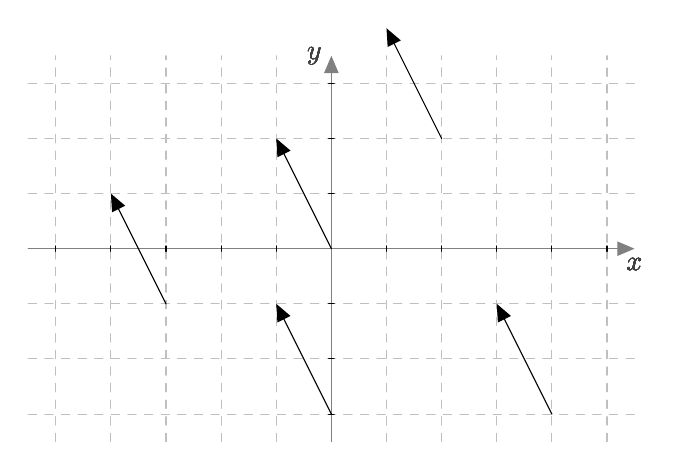
\begin{tikzpicture}[line cap=round,line join=round,>=triangle 45,x=0.7cm,y=0.7cm]

		%x-akseli:
		\draw[->,color=gray] (-5.5,0) -- (5.5,0);
		%tiksut ja viivat
		\foreach \x in {-5,-4,-3,-2,-1,1,2,3,4,5}
		{\draw[dashed, color= lightgray] (\x,-3.5)--(\x,3.5);
		\draw[shift={(\x,0)},color=black] (0pt,1pt) -- (0pt,-1pt);
		\node [below] at (5.5,0) {\textcolor{darkgray}{$x$}};
		}

		%y-akseli
		\draw[->,color=gray] (0,-3.5) -- (0,3.5);

		%tiksut ja viivat
		\foreach \y in {-3,-2,-1,1,2,3}
		{
		\draw[dashed, color=lightgray] (-5.5,\y)--(5.5,\y);
		\draw[shift={(0,\y)},color=black] (1pt,0pt) -- (-1pt,0pt);
		\node [left] at (0,3.5) {\textcolor{darkgray}{$y$}};
		}

		% Varsinainen kuva

		% KOMPONENTTIVEKTORIT

		%\draw[->] (0,0)--(1,0);
		%\node[below] at (0.4, -0.2) {$\vi$};

		%\draw[->] (0,0)--(0,1);
		%\node[left] at (-0.2, 0.4) {$\vj$};

		\draw[->] (2,2)--(1,4);

		\draw[->] (0,-3)--(-1,-1);

		\draw[->] (4,-3)--(3,-1);

		\draw[->] (-3,-1)--(-4,1);

		\draw[->] (0,0)--(-1,2);

	\end{tikzpicture}
	\caption{Vektoreita.}
	\label{kuva:samat erit vektorit}	
	\end{figurehere}
	\end{center}
	
\end{teht}

\maaritelma[Samat vektorit]{\label{maaritelma: samat vektorit} Kaksi vektoria ovat samat, jos ne voidaan esitt�� samalla tavalla vektorien $\vi$ ja $\vj$ avulla.}

Vektorien samuus tarkoittaa siis sit�, ett� ne ovat saman pituisia ja osoittavat samaan suuntaan $-$ niiden paikalla koordinaatistossa ei ole merkityst�.

\begin{teht} Tarkastellaan seuraavaa kuvaa \ref{kuva:paikkavektoreita}. Ilmoita kaikki kuvan vektorit vektorien $\vi$ ja $\vj$ avulla. Vertaa tuloksia vektoreiden k�rkipisteiden koordinaatteihin. Mit� huomaat?

	\begin{center}
	\begin{figurehere}
	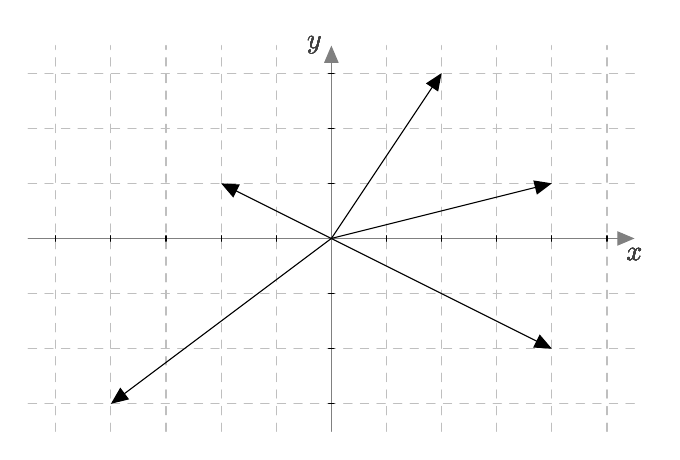
\begin{tikzpicture}[line cap=round,line join=round,>=triangle 45,x=0.7cm,y=0.7cm]

		%x-akseli:
		\draw[->,color=gray] (-5.5,0) -- (5.5,0);
		%tiksut ja viivat
		\foreach \x in {-5,-4,-3,-2,-1,1,2,3,4,5}
		{\draw[dashed, color= lightgray] (\x,-3.5)--(\x,3.5);
		\draw[shift={(\x,0)},color=black] (0pt,1pt) -- (0pt,-1pt);
		\node [below] at (5.5,0) {\textcolor{darkgray}{$x$}};
		}

		%y-akseli
		\draw[->,color=gray] (0,-3.5) -- (0,3.5);

		%tiksut ja viivat
		\foreach \y in {-3,-2,-1,1,2,3}
		{
		\draw[dashed, color=lightgray] (-5.5,\y)--(5.5,\y);
		\draw[shift={(0,\y)},color=black] (1pt,0pt) -- (-1pt,0pt);
		\node [left] at (0,3.5) {\textcolor{darkgray}{$y$}};
		}

		% Varsinainen kuva

		% KOMPONENTTIVEKTORIT

		%\draw[->] (0,0)--(1,0);
		%\node[below] at (0.4, -0.2) {$\vi$};

		%\draw[->] (0,0)--(0,1);
		%\node[left] at (-0.2, 0.4) {$\vj$};

		\draw[->] (0,0)--(2,3);

		\draw[->] (0,0)--(4,1);

		\draw[->] (0,0)--(-2,1);

		\draw[->] (0,0)--(-4,-3);

		\draw[->] (0,0)--(4,-2);

	\end{tikzpicture}
	\caption{Origosta l�htevi� vektoreita.}
	\label{kuva:paikkavektoreita}	
	\end{figurehere}
	\end{center}
	
\end{teht}

\maaritelma[Paikkavektori]{Vektori, joka l�htee origosta ja jonka k�rki on pisteess� $P$, on pisteen $P$ paikkavektori.}

Kuvassa \ref{kuva:paikkavektori} oleva vektori $\vv=4\vi+3\vj$ on siis pisteen $(4,3)$ paikkavektori. 

	\begin{center}
	\begin{figurehere}
	\begin{tikzpicture}[line cap=round,line join=round,>=triangle 45,x=0.7cm,y=0.7cm]

		%x-akseli:
		\draw[->,color=gray] (-5.5,0) -- (5.5,0);
		%tiksut ja viivat
		\foreach \x in {-5,-4,-3,-2,-1,1,2,3,4,5}
		{\draw[dashed, color= lightgray] (\x,-3.5)--(\x,3.5);
		\draw[shift={(\x,0)},color=black] (0pt,1pt) -- (0pt,-1pt);
		\node [below] at (5.5,0) {\textcolor{darkgray}{$x$}};
		}
		
		%y-akseli
		\draw[->,color=gray] (0,-3.5) -- (0,3.5);

		%tiksut ja viivat
		\foreach \y in {-3,-2,-1,1,2,3}
		{
		\draw[dashed, color=lightgray] (-5.5,\y)--(5.5,\y);
		\draw[shift={(0,\y)},color=black] (1pt,0pt) -- (-1pt,0pt);
		\node [left] at (0,3.5) {\textcolor{darkgray}{$y$}};
		}

		% Varsinainen kuva

		% Komponenttivektorit
		\draw[->] (0,0)--(1,0);
		\node[below] at (0.4, -0.2) {$\vi$};

		\draw[->] (0,0)--(0,1);
		\node[left] at (-0.2, 0.4) {$\vj$};

		% Vektorit
		\draw[->] (0,0)--(4,3);
		\node[above left] at (3,2) {$\vv = \textcolor{darkgreen}{4}\vi + \textcolor{blue}{3}\vj$};

		\draw[fill, color = black] (4,3) circle [radius = 1.5pt];
		\node[below right] at (4,3) {$(\textcolor{darkgreen}{4},\textcolor{blue}{3})$};

		% Vektorit
		\draw[->] (0,0)--(-2,-3);
		\node[above left] at (-1.1,-1.7) {$\vw$};
		
	\end{tikzpicture}
	\caption{Pisteen $(4,3)$ paikkavektori $\vv$.}
	\label{kuva:paikkavektori}
	\end{figurehere}
	\end{center}


\begin{teht} Tarkastellaan edelleen kuvaa \ref{kuva:paikkavektori}. 
\begin{aakkosta*}
\item Ilmoita vektori $\vw$ vektorien $\vi$ ja $\vj$ avulla. Mink� pisteen paikkavektori se on?
\item Ilmoita vektorit $\vi$ ja $\vj$ vektorien $\vi$ ja $\vj$ avulla. Mink� pisteiden paikkavektoreita ne ovat?
\end{aakkosta*}
\end{teht}

Tarkastellaan sitten vektoria $0\vi + 0\vj=\bar{0}$. T�t� vektoria sanotaan nollavektoriksi.

\maaritelma[Nollavektori]{Vektoria $0\vi + 0\vj =\bar{0}$ sanotaan nollavektoriksi.}

Nollavektori on siis vektori, jonka alkupiste ja k�rkipiste ovat samat. Nollavektori on my�s origon eli pisteen $(0,0)$ paikkavektori.






\subsection{Kahden pisteen v�linen vektori}

Vektoria pisteest� $A$ pisteeseen $B$ kulkevaa vektoria merkit��n $\pv{AB}$. Vektoria pisteest� $B$ pisteeseen $A$ kulkevaa vektoria merkit��n $\pv{BA}$. 

	\begin{center}
	\begin{figurehere}
	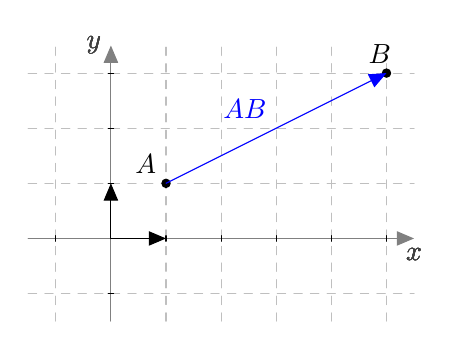
\begin{tikzpicture}[line cap=round,line join=round,>=triangle 45,x=0.7cm,y=0.7cm]
	
		%x-akseli:
		\draw[->,color=gray] (-1.5,0) -- (5.5,0);
		%tiksut ja viivat
		\foreach \x in {-1,1,2,3,4,5}
		{\draw[dashed, color= lightgray] (\x,-1.5)--(\x,3.5);
		\draw[shift={(\x,0)},color=black] (0pt,1pt) -- (0pt,-1pt);
		\node [below] at (5.5,0) {\textcolor{darkgray}{$x$}};
		}
		
		%y-akseli
		\draw[->,color=gray] (0,-1.5) -- (0,3.5);

		%tiksut ja viivat
		\foreach \y in {-1,1,2,3}
		{
		\draw[dashed, color=lightgray] (-1.5,\y)--(5.5,\y);
		\draw[shift={(0,\y)},color=black] (1pt,0pt) -- (-1pt,0pt);
		\node [left] at (0,3.5) {\textcolor{darkgray}{$y$}};
		}

		% Varsinainen kuva

		% Komponenttivektorit
		\draw[->] (0,0)--(1,0);
		\node[below] at (0.4, -0.2) {$\vi$};

		\draw[->] (0,0)--(0,1);
		\node[left] at (-0.2, 0.4) {$\vj$};

		% Vektorit

		\draw[fill, color = black] (1,1) circle [radius = 1.5pt];
		\node[above left] at (1,1) {$A$};
		
		\draw[fill, color = black] (5,3) circle [radius = 1.5pt];
		\node[above right] at (4.5,3) {$B$};

		\draw[->, color=blue] (1,1)--(5,3);
		\node[above left] at (3,2) {\textcolor{blue}{$\pv{AB}$}};

	\end{tikzpicture} % pic 1
	\hspace{0.7cm}
	\begin{tikzpicture}[line cap=round,line join=round,>=triangle 45,x=0.7cm,y=0.7cm]
	
		%x-akseli:
		\draw[->,color=gray] (-1.5,0) -- (5.5,0);
		%tiksut ja viivat
		\foreach \x in {-1,1,2,3,4,5}
		{\draw[dashed, color= lightgray] (\x,-1.5)--(\x,3.5);
		\draw[shift={(\x,0)},color=black] (0pt,1pt) -- (0pt,-1pt);
		\node [below] at (5.5,0) {\textcolor{darkgray}{$x$}};
		}
		
		%y-akseli
		\draw[->,color=gray] (0,-1.5) -- (0,3.5);

		%tiksut ja viivat
		\foreach \y in {-1,1,2,3}
		{
		\draw[dashed, color=lightgray] (-1.5,\y)--(5.5,\y);
		\draw[shift={(0,\y)},color=black] (1pt,0pt) -- (-1pt,0pt);
		\node [left] at (0,3.5) {\textcolor{darkgray}{$y$}};
		}

		% Varsinainen kuva

		% Komponenttivektorit
		\draw[->] (0,0)--(1,0);
		\node[below] at (0.4, -0.2) {$\vi$};

		\draw[->] (0,0)--(0,1);
		\node[left] at (-0.2, 0.4) {$\vj$};

		% Vektorit

		\draw[fill, color = black] (1,1) circle [radius = 1.5pt];
		\node[above left] at (1,1) {$A$};
		
		\draw[fill, color = black] (5,3) circle [radius = 1.5pt];
		\node[above right] at (4.5,3) {$B$};

		\draw[->, color=darkgreen] (5,3)--(1,1);
		\node[below right] at (2.5,2) {\textcolor{darkgreen}{$\pv{BA}$}};

	\end{tikzpicture}
	\caption{Kahden pisteen v�liset vektorit.}
	\label{kuva:kahden pisteen v�linen vektori}
	\end{figurehere}
	\end{center}


\begin{teht} ...
\begin{aakkosta*}
\item Piirr� koordinaatisto ja valitse sen ensimm�iselt� nelj�nnekselt� kaksi pistett�. Merkitse n�it� pisteit� kirjaimilla $P$ ja $Q$. Merkitse my�s pisteiden koordinaatit n�kyviin.
\item Piirr� vektori $\pv{PQ}$. 
\item Ilmoita vektori $\pv{PQ}$ vektorien $\vi$ ja $\vj$ avulla. 
\end{aakkosta*}
\end{teht}

\begin{teht} ...
\begin{aakkosta*}
\item Piirr� koordinaatisto ja valitse sen toiselta, kolmannelta tai nelj�nnekselt� nelj�nnekselt� kaksi pistett�. Merkitse n�it� pisteit� kirjaimilla $R$ ja $S$. Merkitse my�s pisteiden koordinaatit n�kyviin.
\item Piirr� vektori $\pv{RS}$. 
\item Ilmoita vektori $\pv{RS}$ vektorien $\vi$ ja $\vj$ avulla. 
\end{aakkosta*}
\end{teht}
	
\begin{teht} ...
\begin{aakkosta*}
\item Piirr� koordinaatistoon jotkin pisteet $A$ ja $B$. Merkitse niiden koordinaatit.
\item Ilmoita vektori $\pv{AB}$ vektorien $\vi$ ja $\vj$ avulla. 
\item Ilmoita vektori $\pv{BA}$ vektorien $\vi$ ja $\vj$ avulla. 
\item Vertaa b- ja c-kohdan tuloksia. Mit� huomaat?
\end{aakkosta*}
\end{teht}
	
Vektorit $\pv{AB}$ ja $\pv{BA}$ ovat eri vektorit, sill� niit� ei voida esitt�� samalla tavalla vektorien $\vi$ ja $\vj$ avulla. Vektorin suunnalla on siis merkityst�. Vektorien suuntiin palataan kappaleessa \ref{subsebtion:vektorien kertominen reaaliluvulla}.  	







































\begin{comment}
\begin{teht} Tarkastellaan alla olevaa kuvaa \ref{kuva:kaksi samaa vektoria}.
	
% KUVA
		\begin{center}
		\begin{figurehere}
	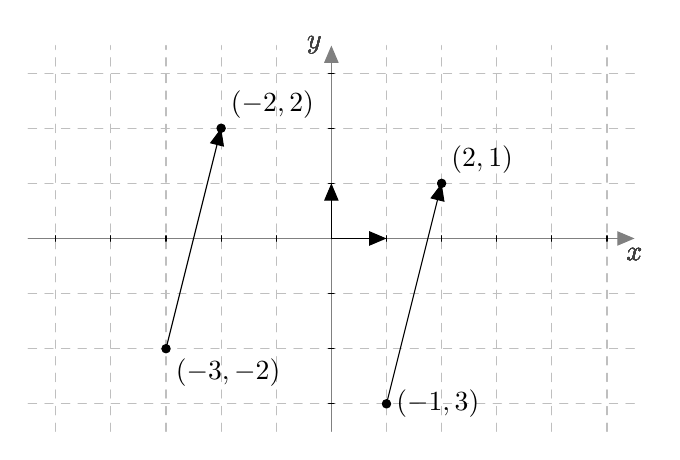
\begin{tikzpicture}[line cap=round,line join=round,>=triangle 45,x=0.7cm,y=0.7cm]

		%x-akseli:
		\draw[->,color=gray] (-5.5,0) -- (5.5,0);
		%tiksut ja viivat
		\foreach \x in {-5,-4,-3,-2,-1,1,2,3,4,5}
		{\draw[dashed, color= lightgray] (\x,-3.5)--(\x,3.5);
		\draw[shift={(\x,0)},color=black] (0pt,1pt) -- (0pt,-1pt);
		\node [below] at (5.5,0) {\textcolor{darkgray}{$x$}};
		}


		%y-akseli
		\draw[->,color=gray] (0,-3.5) -- (0,3.5);

		%tiksut ja viivat
		\foreach \y in {-3,-2,-1,1,2,3}
		{
		\draw[dashed, color=lightgray] (-5.5,\y)--(5.5,\y);
		\draw[shift={(0,\y)},color=black] (1pt,0pt) -- (-1pt,0pt);
		\node [left] at (0,3.5) {\textcolor{darkgray}{$y$}};
		}

		% Varsinainen kuva

		% KOMPONENTTIVEKTORIT
		\draw[->] (0,0)--(1,0);
		\node[below] at (0.4, -0.2) {$\vi$};

		\draw[->] (0,0)--(0,1);
		\node[left] at (-0.2, 0.4) {$\vj$};
		
		% pisteet
		\draw[fill, color = black] (-3,-2) circle [radius = 1.5pt];
		\node[below right] at (-3,-2) {$(-3,-2)$};		
		
		\draw[fill, color = black] (-2,2) circle [radius = 1.5pt];
		\node[above right] at (-2,2) {$(-2,2)$};

		\draw[fill, color = black] (2,1) circle [radius = 1.5pt];
		\node[above right] at (2,1) {$(2,1)$};

		\draw[fill, color = black] (1,-3) circle [radius = 1.5pt];
		\node[right] at (1,-3) {$(-1,3)$};

		% vektorit
		\draw[->] (-3,-2)--(-2,2);
		\node[left] at (-3, 0.5) {$\vv$};

		\draw[->] (1,-3)--(2,1);
		\node[right] at (2, -0.5) {$\vw$};
		

	\end{tikzpicture}
	\caption{Vektoreita}
	\label{kuva:kaksi samaa vektoria}	
		\end{figurehere}
		\end{center}
	
	
		\begin{aakkosta*}
		\item Ilmoita vektori $\vv$ vektorien $\vi$ ja $\vj$ avulla. 
		\item Ilmoita vektori $\vw$ vektorien $\vi$ ja $\vj$ avulla.
		\item Mit� huomaat?
		\end{aakkosta*}
	\end{teht}
\end{comment}











\end{document}